\chapter{Zdroje dát pre analýzu}
\label{data-sources-available-for-research}

% # PART 2
% # TODO obsah by mal napovedat, ze vysledky boli dosiahnute
%        nejčastěji navštěvovaných stránek
%        Selenium
%        výhody a nevýhody vlastnych a externych dat
% # TODO sekcia o automatizovanom prehliadani stranok, Playwright
% # TODO nie je az tak dolezite, ze su najnavstevovanejsie, ako ze sa to automatizuje
% # TODO spomenut ale aj Selenium

Poznávacím znamením využívania technológie NEL je prítomnosť hlavičiek \code{NEL} a \code{Report-To} v HTTP odpovediach z monitorovaných web serverov. 
Pre účely analýzy jej využívania je teda nutné získať dáta obsahujúce tieto odpovede.
Cieľom je pozerať sa buď na reálne komunikácie, ktoré už prebehli, alebo skúmať ako web servery aktuálne dosiahnuteľné na internete
odpovedajú na HTTP požiadavky. 
V tejto kapitole sú detailne popísané dostupné zdroje dát a konkrétne spôsoby, akými možno záznamy takýchto komunikácií získať.

\section{Potrebné dáta}

V prvom rade je nutné definovať množinu webových serverov, pre ktoré možno získať potrebné záznamy HTTP komunikácie.
Vzhľadom na to, že web servery možno adresovať pomocou ich doménového mena, ďalej tieto web servery označujem ako skúmané domény.
Množinu skúmaných domén možno zaobstarať z niekoľkých zdrojov, ktoré sú popísané v sekcií \ref{tranco}.

Po definovaní množiny skúmaných domén je možné zmienené záznamy o komunikácií s nimi získať podľa toho, kedy komunikácia prebehla:
\begin{enumerate}
    \item Súčasnosť -- aktuálne dáta:
    
    Z hľadiska prítomnosti je možné použiť napríklad techniku automatizovaného webového prehliadania.
    Na účel toho je možné použiť už existujúce technológie ako Selenium alebo Playwright, ktoré opisuje sekcia \ref{selenium}.

    \item Minulosť -- historické dáta:

    Pre sledovanie historického vývoja nasadenia NEL je tiež nevyhnutné nahliadnuť do histórie prevádzky skúmaných domén. 
    Z tohto hľadiska je nutné použiť už spracované a uložené dáta. 
    Vyhovujúcim zdrojom historických dát je napríklad projekt \textbf{HTTP Archive}, ktorému sa táto práca venuje primárne, a to v sekcií \ref{httparchive}.
    Ide o službu, ktorá zaznamenáva vývoj webu od roku 2010 a teda jej vhodnosť sa potvrdzuje tým, že špecifikácia NEL v tejto práci bola publikovaná až v roku 2018.
\end{enumerate}

\pagebreak

\section{Množina skúmaných domén}
\label{tranco}

% Platí, že čím je mohutnejšia množina skúmaných domén, tým presnejšiu analýzu využívania NEL na webe možno vypracovať.
% Preto je pri výbere takejto množiny kľúčová jej mohutnosť.
Existujú projekty, ktoré sa zaoberajú získavaním doménových mien pre rôzne účely.
Niektoré sú vypracované na to aby uchovávali tie, ktorých webstránky sú najčastejšie navšetevované \cite{hacker-target-website-lists-overview, tranco}.
Iné projekty zase spravujú zoznam tých, ktoré navštevujú používatelia iných služieb autorov daného projektu \cite{chrome-crux}. 

\subsection{Najčastejšie navštevované domény}

Jeden z projektov, ktorých účelom je zaznamenávanie domén s najčastejšie navštevovanými webstránkami je TRANCO \cite{tranco}.
Projekt TRANCO poskytuje sadu nástrojov pre generovanie rebríčkov najpopulárnejších domén. 
Tieto rebríčky webových domén zoradených podľa hodnotenia návštevnosti ich webstránok je odolný proti externej manipulácií a vhodný na účely výskumu. 
Vznikol na základe častej potreby pre skúmanie práve takýchto domén či už pre jednoduchú referenciu, alebo ako podklad pre ďalší prieskum.
TRANCO nie je prvým takýmto rebríčkom, ale je prvým, ktorý sa zaoberá nedostatkami iných existujúcich rebríčkov.
Existujúce rebríčky využíva ako zdroje dát pre tvorbu toho svojho.
Nový rebríček TRANCO sa tvorí zlučovaním zdrojových rebríčkov do nového, stabilnejšieho rebríčka, ktorý reprezentuje domény v globálnej škále.
TRANCO dokonca do určitej miery odstraňuje zo zdrojových rebríčkov domény, na ktorých môže byť zverejnený nežiadúci (nebezpečný) obsah.
Obsahuje primárne registrovateľné domény, čo sú domény, ktoré si môže priamo zakúpiť či už jednotlivec alebo organizácia. 
Príkladom môžu byť domény registrované pod TLD \code{com}, ale aj domény registrované pod eTLD zo zoznamu verejných suffixov ako \mbox{\code{co.uk} \cite{tranco}}.

TRANCO je podložený štúdiom zameraným na vylepšenie dostupných alternatív rebríčkov populárnych domén.
Práve tieto alternatívne rebríčky tvoria vnútorne použité zdroje dát pre výsledné rebríčky TRANCO.
Medzi ne patria projekty \cite{tranco-config}:
\begin{itemize}
    \item Alexa Top Sites,
    \item Majestic Million,
    \item Cisco Umbrella,
    \item Quantcast,
    \item Chrome User Experience Report,
    \item Cloudflare Radar.
\end{itemize}
TRANCO je ako zdroj skúmaných domén pre túto prácu vhodný, pretože sprístupňuje a vylepšuje presnosť záznamov z týchto alternatív.
Taktiež udržiava ich historické dáta, ktoré už nie sú samostatne dostupné.
Vzhľadom na to je možné preskočiť výber toho najvhodnejšieho z pomedzi nich a použiť práve TRANCO.

\subsubsection{Generovanie rebríčka TRANCO}
\label{tranco-generation}

V jeho štandardnej forme, rebríček TRANCO sa generuje každý deň v dvoch verziách:
\begin{itemize}
    \item TRANCO rebríček domén
    \item TRANCO rebríček domén a subdomén
\end{itemize}

V tomto každodenne generovanom rebríčku sú prednastavené aj zdroje dát, teda použité zdrojové rebríčky, aj dátumový rozsah, za ktorý sa zo zdrojových rebríčkov má čerpať.
Štandardne sa vytvára výsledok z rebríčkov Chrome User Experience Report, Majestic Million, Cloudflare Radar a Cisco Umbrella.
Dátumový rozsah je nastavený na posledných 30 dní \cite{tranco-config}, pričom TRANCO použije ako kompletný zdroj dát všetky spomenuté rebríčky vygenerované za túto dobu. 

V novom TRANCO rebríčku sa zo zdrojových rebríčkov spriemeruje pre každú doménu jej zaradenie aplikovaním jednej z dostupných kombinačných metód pre upravenie finálneho hodnotenia domén.
Pre štandardný rebríček je využitá kombinačná metóda takzvanej harmonickej progresie, nazývaná Dowdall rule. 
Dowdall rule hodnotí v zozname obsahujúcom N domén prvú hodnotou 1 a všetky ostatné postupne \(1/2\), \(1/3\) až \(1/(N-1)\) a zakončí hodnotením poslednej -- \(1/N\) \cite{tranco, tranco-config}.
Názornú ukážku aplikovania Dowdall rule na rebríčky vizualizuje obrázok \ref{img:dowdall-rule}.
Generuje sa v ňom nový rebríček o veľkosti štyroch domén, takže sa do úvahy beriú prvé štyri domény z každého vstupného rebríčka. 
Skóre sa vypočíta podľa umiestnenia a podľa celkového počtu domén radených v danom zdrojovom rebríčku. 
Rebríček 4 (v obrázku úplne napravo) s najvyšším počtom hodnotených domén výsledok ovplyvnil najviac.

\begin{figure}[htb]
\begin{center}
 % 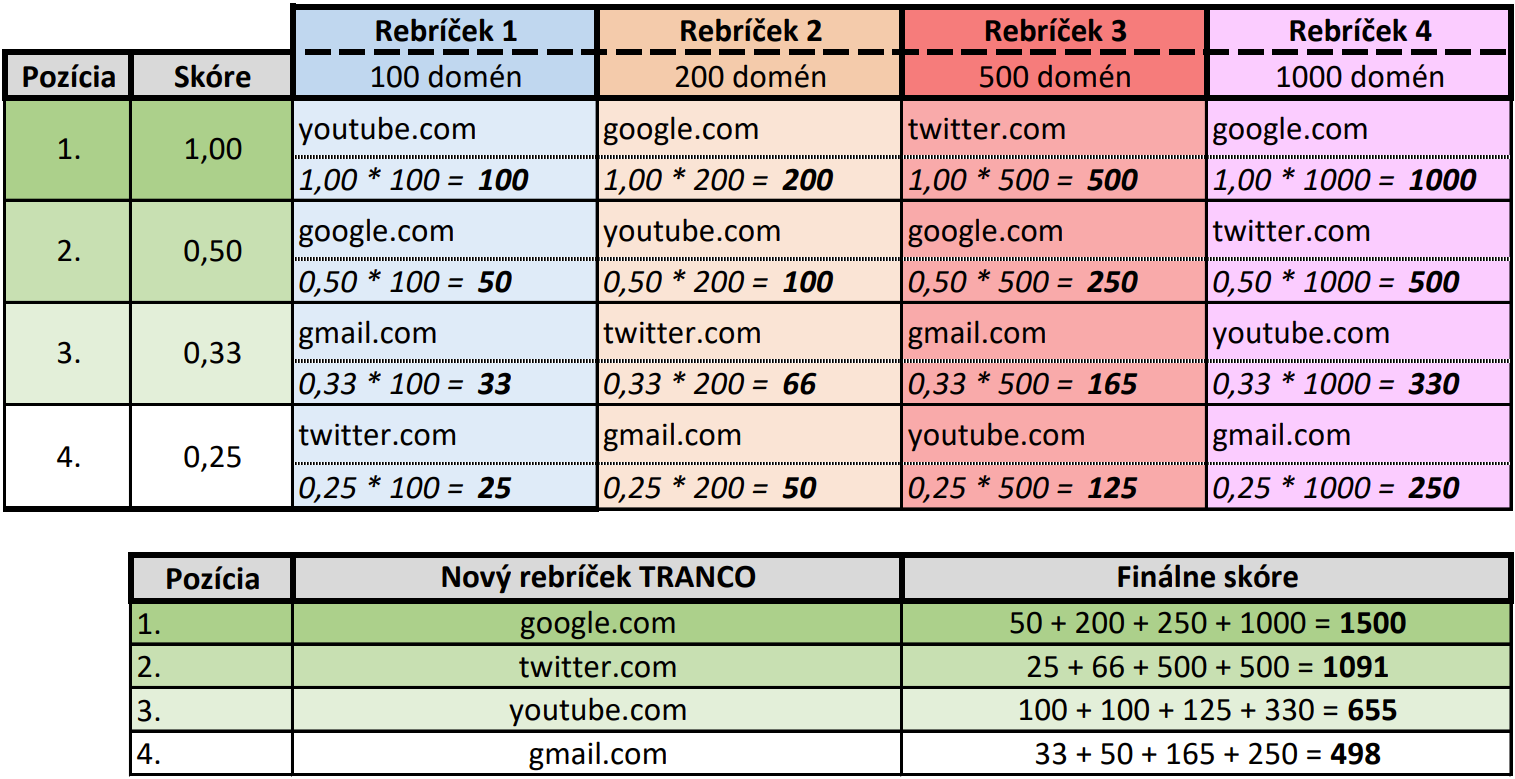
\includegraphics[scale=0.375]{obrazky-figures/dowdall_rule.png}
 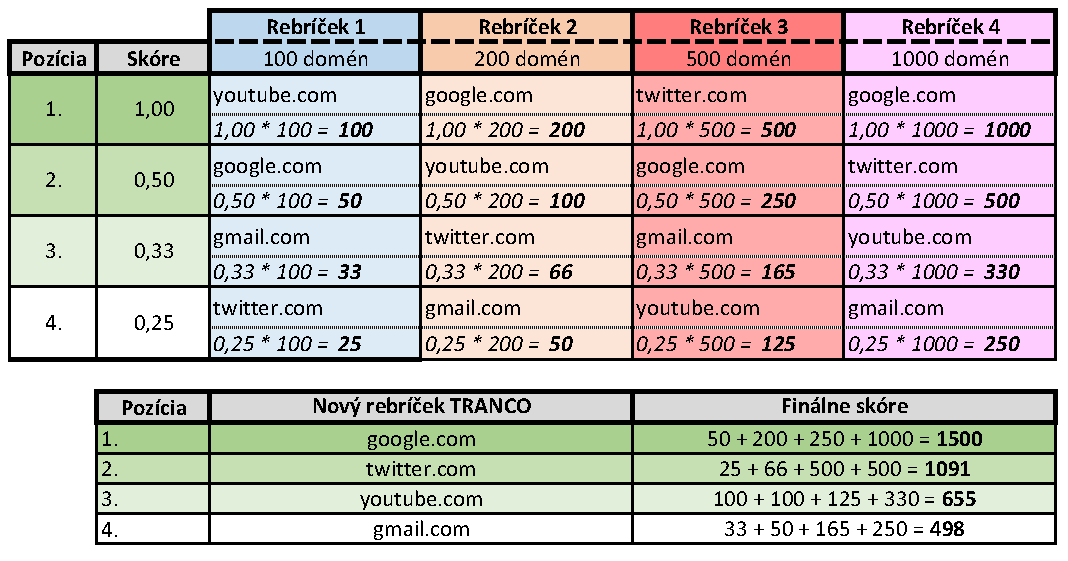
\includegraphics[scale=0.84]{obrazky-figures/dowdall_rule_size_fit_cropped.pdf}
 \caption{\centering Príklad uplatnenia Dowdall rule na spriemerovanie štyroch vstupných rebríčkov do výsledného rebríčka TRANCO.}
 \label{img:dowdall-rule}
\end{center}
\end{figure}

Po dokončení priemerovania a zoraďovania sa spolu s výsledným rebríčkom vytvorí na oficiálnom webe TRANCO aj jedinečná stránka obsahujúca odkaz na jeho stiahnutie a tiež citácia, 
ktorou je možné jedinečne odkazovať na tento nový rebríček v prácach, ktoré ho môžu použiť na svoje účely.
Zároveň, okrem generovania nových TRANCO rebríčkov sú na oficiálnej stránke dostupné aj historicky vygenerované, spomenuté štandardné, každodenné rebríčky \cite{tranco-homepage}.

Príklad obsahu vygenerovaného rebríčka znázorňuje výpis \ref{listing:tranco-obsah}.
Rebríček je možné stiahnuť vo formáte \code{zip} archívu, ktorý obsahuje práve jeden súbor nazvaný \textbf{top-1m.csv}. 
Obsahom je na každom riadku čiarkou oddelené umiestnenie domény a jej meno.

\pagebreak

\begin{center}
\centering
\begin{lstlisting}[
caption={\centering Ukážka vygenerovaného denného rebríčku z 12. januára 2024, orezaného na prvých 10 domén.},
label=listing:tranco-obsah, 
language=json, 
frame=lb,
xleftmargin=.3875\textwidth, 
xrightmargin=.3875\textwidth]
1,google.com
2,amazonaws.com
3,facebook.com
4,microsoft.com
5,a-msedge.net
6,googleapis.com
7,apple.com
8,youtube.com
9,akamaiedge.net
10,akamai.net

\end{lstlisting}
\end{center}

\subsection{Domény navštevované používateľmi prehliadača Google Chrome}
\label{chrome-user-experience-report}


\section{Automatizované prehliadanie webu}
\label{selenium}

Táto sekcia ešte nie je napísaná.

% Web Crawling je technika skúmania webu, ktorá programovo vstúpi na zvolenú stránku a získava o nej informácie ako metadáta, jej obsah a iné dáta v oblasti záujmu \cite{httparchive-webcrawling}.

\section{HTTP Archive}
\label{httparchive}

Projekt HTTP Archive sa zaoberá zaznamenávaním spôsobu konštrukcie a poskytovania digitálneho obsahu na webe. Je permanentným repozitárom informácií o webe a udržiava záznamy ako veľkosti
stránok, zlyhané HTTP požiadavky alebo technológie využité v rámci konkrétnej stránky. Vďaka týmto dátam je možné pozorovať trendy v histórií vývoja webu ako celku a zároveň je nad nimi možné vykonávať
rôzne podrobné prieskumy a analýzy \cite{httparchive-about}. 

Autormi HTTP Archive sú členovia komunity zvanej Web Performance Group. Pôvodným autorom je Steve Souders, ktorý projekt založil v roku 2010 \cite{httparchive-faq}.
Momentálne sa na jeho údržbe po stránke vývoja podieľa štvorica hlavných členov, a keďže ide o open source projekt, v prevádzke ho udržiavajú sponzori ako aj spoločnosti Google, Mozilla, O'Reilly Media a Fastly.
Taktiež je tento projekt súčasťou projektu Internet Archive, ktorý už od roku 1996 slúži ako digitálna knižnica poskytujúca prístup ku knihám, filmom, hudbe a rovnako aj k miliardám archivovaných webstránok \cite{httparchive-about}.

Cieľom projektu je vytvoriť a udržiavať služby poskytujúce možnosť nahliadnuť do histórie webu, pozorovať jeho prechod do momentálneho stavu a vďaka získaným poznatkom dokázať
predpovedať potencionálne nové trendy blízkej budúcnosti. 
Pre tento účel vyvinuli sadu nástrojov pre zbieranie uvedených dát z webu, efektívne ukladanie nadobudnutých dát a ich reprezentáciu na svojej webovej stránke.
Na uskladnenie dát sa používa služba \mbox{\textbf{BigQuery} poskytovaná} na platforme \textbf{Google Cloud Platform} (ďalej už iba GCP).
Tieto dáta sú verejne prístupné ako databázové tabuľky v prostredí BigQuery.
Prehliadať ich možno pomocou príkazov jazyka Structured Query Language, zaužívaného štruktúrovaného jazyka pre správu dát uložených v databáze (ďalej ako SQL).

Vhodnosť projektu pre túto prácu spočíva v tom, že ide o komunitný projekt, ktorého výsledky sú verejne dostupné. 
Keďže umožňuje prístup k historickým záznamom reálneho prenosu HTTP komunikácie na webe, ktoré siahajú až po rok 2010, prirodzene sa z neho stáva primárny zdroj pre výskumy a analýzy, akou je aj analýza v rámci tejto práce.


\subsection{Získavanie dát}
\label{fetching-data}

Ako bolo zmienené, HTTP Archive získava dáta z webu. 
Získava ich pomocou automatizovaného prehliadania webu (viď sekciu \ref{selenium}).
Cieľové dáta predstavujú celkový aplikačný prenos na prehliadaných doménach, kde meranou dátovou jednotkou je HTTP žiadosť a HTTP odpoveď, ktorou na žiadosť daná doména zareaguje.
Keďže môžu nastať odlišnosti v komunikácií vedenej z bežného počítača oproti takej, ktorá je vedená z mobilného zariadenia, HTTP Archive zaznamenáva výsledky aj z počítačového (\textbf{desktop}), aj z \textbf{mobilného} prostredia.
Zo získaných dát potom svojimi algoritmami extrahuje všetky dôležité poznatky, medzi ktoré patria napríklad aj stránkou používané zdroje a použité webové aplikačné rozhrania (Web API) \cite{httparchive-homepage}.

Ako zoznam vstupných domén do tohto procesu HTTP Archive momentálne používa projekt Chrome User Experience Report, popísaný v sekcii \ref{chrome-user-experience-report}.

\subsubsection{WebPageTest}

Nástroj použitý pre automatizované prehliadanie webu je WebPageTest. Tento nástroj (ďalej označovaný už iba ako WPT) je softvér na testovanie výkonnosti webstránok vyvinutý spoločnosťou Google \cite{webpagetest}. 
Predstavuje komplexné riešenie schopné merať rôzne metriky ako proces načítavania, vykresľovania a využitia siete pre vybrané web stránky. 
Je zverejnený priamo na stránkach jeho oficiálneho repozitára GitHub\footnote{\href{https://github.com/catchpoint/WebPageTest}{https://github.com/catchpoint/WebPageTest}} spolu s priloženou dokumentáciou, a to pod open source licenciou.

HTTP Archive na svoje účely používa vlastnú WPT inštanciu. 
Táto inštancia je priebežne synchronizovaná s najnovšou dostupnou verziou.
Vo svojich behoch využíva doplnkovú funkcionalitu WPT --- vlastné (prispôsobené) metriky.
Pridanie vlastných metrík do WPT predstavuje spúšťanie ľubovolnej funkcie napísanej v jazyku JavaScript na konci behu testovania danej webstránky. 
Použitím tejto funkcionality HTTP Archive dokáže zbierať akékoľvek dodatočne vypočítané metriky z webstránok domén, pre ktoré zbiera \mbox{dáta \cite{webpagetest}}.

Je dôležité poznamenať, že stránky sú testované s čistou vyrovnávacou pamäťou cache. 
Taktiež sa na stránkach vyžadujúcich autentifikáciu nikdy neprihlasuje.
To môže spôsobovať odchýlku oproti reálnemu scenáru používania navštevovaných web stránok. 
WPT je spúšťaný vždy prvý deň v mesiaci, takže HTTP Archive zverejňuje dáta na mesačnej báze.

Pre účely uskladňovania získaných dát je využitý formát HTTP Archive súboru (prípona \code{.har}, ďalej označovaný už len ako HAR).
Formát HAR je prispôsobený na uskladňovanie dát spojenia nadviazanom vo webovom prehliadači. Samotné dáta sú serializované vo formáte JSON.
Bežným obsahom HAR súboru býva HTTP žiadosť, prislúchajúca odpoveď, metriky výkonnosti načítania stránky a iné \cite{httparchive-harfile}. 
Orientačný príklad obsahu takéhoto súboru je vo výpise \ref{listing:harfile}.
Všetky detaily týkajúce sa procesu získania webstránky sú zaznamenané v položke \code{log}. Pole \code{version} definuje verziu súboru HAR. Pole \code{pages} obsahuje napríklad URL získaného zdroja a pole \code{entries} obsahuje HTTP žiadosti \mbox{a odpovede pre daný zdroj a zdroje ním používané.}

\pagebreak

\begin{center}
\centering
\begin{lstlisting}[
caption={\centering Orientačná ukážka obsahu súboru HAR.},
label=listing:harfile, 
language=json, 
frame=tb,
xleftmargin=.09\textwidth, 
xrightmargin=.09\textwidth]
{
  "log": {
    "version": "1.2",
    ...
    "pages": [
      {
        "startedDateTime": "2024-01-12T15:25:01.278Z",
        "id": "page_1",
        "title": "https://tranco-list.eu/list/KJ49W/1000000",
        "pageTimings": {...}
      }
    ],
    "entries": [
      {
        ...
        "request": {...},
        "response": {...},
        ...
      },
      ...
    ]
  }
}
\end{lstlisting}
\end{center} 

\subsection{Ukladanie dát}

Dáta získané pomocou WPT sa nahrávajú do existujúcich databázových tabuliek prostredia BigQuery, čím sú sprístupnené pre prehliadanie \cite{httparchive-faq}.

\subsubsection{BigQuery}
\label{big-query}

BigQuery, infraštruktúra pre ukladanie dát v rámci GCP, je produkt, ktorý umožňuje jeho užívateľom spravovať a analyzovať dáta za pomoci vstavaných funkcionalít ako napríklad aj strojového učenia.
BigQuery je samo o sebe riešenie populárne označované ako platforma poskytovaná ako služba (PaaS).
Hlavnou výhodou pre užívateľov služby typu PaaS je, že sa nemusia nijako starať o správu infraštruktúry, pod čím sa vlastne myslí daná platforma, kde je služba sprevádzkovaná.
O správu potrebnej infraštruktúry (servery, sieťové prvky, bezpečnosť) sa stará GCP, teda poskytovateľ tejto služby.
Tým pádom je možné BigQuery ako úložisko dát veľmi rýchlo zakomponovať do akéhokoľvek vlastného projektu \cite{google-bq}.

Dôležitou vlastnosťou Big Query je prispôsobenosť na vysokorýchlostné výpočty nad obrovským množstvom dát.
Distribúcia výpočtov umožňuje docieliť vykonávanie analýzy nad dátami o veľkosti v terabajtoch za sekundy (TB/s) a petabajtoch za minúty (PB/m).
K tomu napomáha špeciálna vnútorná reprezentácia uložených tabuliek. 
Bežný spôsob ukladania dát do tabuliek v databáze je takzvaný riadkovo orientovaný.
Orientovanie na riadky znamená, že sa záznamy v tabuľke ukladajú priamo vedľa seba na disk databázy.
To je vhodné pre prípady, keď sú na úložisku záznamy vyhľadávané individuálne.
Avšak, pre zložité analytické výpočty nad veľkým objemom dát to predstavuje problém vo výkonnosti, pretože sa musia potupne pre každý záznam tabuľky prehľadať všetky jeho polia \mbox{(stĺpce) \cite{google-bq}}.

\begin{figure}[htb]
\begin{center}
 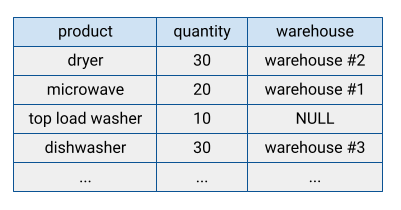
\includegraphics[scale=0.7]{obrazky-figures/row-oriented-store.png}
 \caption{\centering Vizualizácia uskladnenia dát v riadkovo orientovanej databáze.}
 \label{img:row-oriented-store}
\end{center}
\end{figure}

Riešenie, ktorým BigQuery tento problém adresuje je použitie orientácie na jednotlivé stĺpce. 
Ukladaním dát v stĺpcovom formáte, a teda ukladaním každého stĺpca separátne umožňuje prehľadávať dataset bez viazania sa na všetky ostatné stĺpce.
Tým sa efektívne znižuje množstvo dát, ktoré sa prehľadávajú naraz.
Takto je databáza optimalizovaná pre analýzy nad obrovským množstvom uložených záznamov \cite{google-bq}.

\begin{figure}[htb]
\begin{center}
 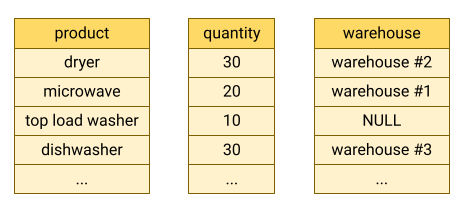
\includegraphics[scale=0.7]{obrazky-figures/column-oriented-store.png}
 \caption{\centering Vizualizácia uskladnenia dát s využitím orientácie na jednotlivé stĺpce.}
 \label{img:column-oriented-store}
\end{center}
\end{figure}

Dáta skladované v BigQuery sú organizované do skupín klasických databázových tabuliek nazývaných dataset.
Je dostupné množstvo datasetov pre prehľadávanie.
Najprv je ale nutné založiť si Google Cloud projekt na oficiálnej stránke, ktorý slúži ako priestor mien pre zdroje, ktoré užívateľ do projektu pridáva a používa.
K dátam je možné priamo pristupovať prostredníctvom troch rozhraní \cite{google-cloud}:
\begin{enumerate}
    \item Google Cloud Console:

    Webové grafické rozhranie pre spravovanie Google Cloud projektov. 
    Časť Google Cloud Console, ktorú užívatelia môžu využiť špecificky na prehliadanie dát BigQuery sa nazýva \textbf{BigQuery Studio}.
    Výhodou tohto spôsobu pracovania so zdrojmi je vysoká úroveň interaktivity, ktorú ponúka zabudované integrované vývojové prostredie pre prácu s dátami. 

    \item BigQuery nástroj príkazového riadku:

    Pre zobrazovanie databáz a tabuliek, prehľadávanie a spravovanie dát v prostredí príkazového riadka je možné využiť nástroj s názvom \code{bq}. 
    
    \item BigQuery klientske knižnice

    Vďaka klientským knižniciam implementujúcim komunikačné rozhranie s BigQuery je taktiež dostupná možnosť programovo manipulovať a prehliadať zdroje priradené ku Google Cloud projektu používateľa.
    Táto možnosť je vhodná pre predom definované, opakované úlohy, ktoré či už požadujú zdroje na vstupe, alebo ich počas svojho behu nahrávajú, prípadne upravujú podľa potreby.
\end{enumerate}

Pri využití ktorejkoľvek z týchto možností platí, že prehliadanie a manipuláciu dát umožňuje jazyk SQL \cite{google-bq}.
V prostredí BigQuery sa používa dialekt pre SQL nazývaný \textbf{GoogleSQL}\footnote{\href{https://cloud.google.com/bigquery/docs/reference/standard-sql/query-syntax}{https://cloud.google.com/bigquery/docs/reference/standard-sql/query-syntax}}.
Ako už bolo uvedené, HTTP Archive ukladá svoje výstupné dáta práve do BigQuery.
Tieto dáta možno nájsť pomocou Google Cloud Console dostupné ako \textbf{zdroj} (anglicky resource), ktorý si môže prihlásený používateľ pridať do svojho projektu.
Po pridaní tohto zdroja s priradeným názvom \code{httparchive} do projektu\footnote{\href{https://github.com/HTTPArchive/httparchive.org/blob/main/docs/gettingstarted\_bigquery.md}{https://github.com/HTTPArchive/httparchive.org/blob/main/docs/gettingstarted\_bigquery.md}} sa sprístupnia pre používanie datasety ako napríklad \cite{httparchive-repo}:

\begin{itemize}
    \item \code{summary\_pages}:

    Obsahuje detaily o jednotlivých web stránkach ako časy ich načítania, počet žiadostí o jej zdroje, typy zdrojov a ich veľkosti.
    Taktiež sú tu informácie týkajúce sa presmerovaní, vzniknutých chýb, použitých služieb ako CDN\footnote{\href{https://www.cloudflare.com/learning/cdn/what-is-a-cdn/}{https://www.cloudflare.com/learning/cdn/what-is-a-cdn/}} a iné.
    
    \item \code{summary\_requests}:

    Nachádzajú sa tu dáta o konkrétnych objektoch načítaných ako už spomínané zdroje pre web stránky v datasete \code{summary\_pages}.
    V dátach je možné prehľadávať ako boli zdroje načítané priamo v hlavičkách HTTP odpovede, v ktorej prišli zo serveru poskytujúceho danú stránku.
    
    \item \code{pages}:

    Extrahované HAR súbory pre každú URL z prehľadávaných web stránok.
    
    \item \code{requests}:

    Extrahované HAR súbory pre každý zdroj jednotlivých prehľadávaných web sránok \mbox{v \code{pages} datasete}.
    
    \item \code{response\_bodies}:

    Extrahované HAR súbory obsahujúce celé telo HTTP odpovede z každej URL prehľadávaných web stránok.
    Ide o veľmi veľké tabuľky, ktoré môžu dosahovať veľkosť \mbox{v jednotkách terabajtov (TB)}.
\end{itemize}

BigQuery zdroj \code{httparchive} sprístupňuje aj niekoľko ďalších datasetov. Táto práca sa jednoznačne najviac zaoberá datasetom \code{summary\_requests}.

Každý z týchto datasetov obsahuje tabuľky nazvané podľa rovnakej konvencie --- dátum vykonaného zberu dát a prostredie, v akom prebiehal.
Dátum je definovaný formátom \code{YYYY\_MM\_DD}, kde \code{YYYY} predstavuje rok, \code{MM} mesiac a \code{DD} deň. 
Prostredie môže byť buď počítačové alebo mobilné, ako sa spomína už v sekcii \ref{fetching-data}.
Príkladom názvu tabuľky teda môže byť \code{2018\_01\_15\_mobile} alebo \code{2023\_01\_01\_desktop}.
Za použitia GoogleSQL je možné tabuľky kombinovať a vytvárať komplexné sady dát pre ďalšiu analýzu.

\begin{figure}[htb]
\begin{center}
 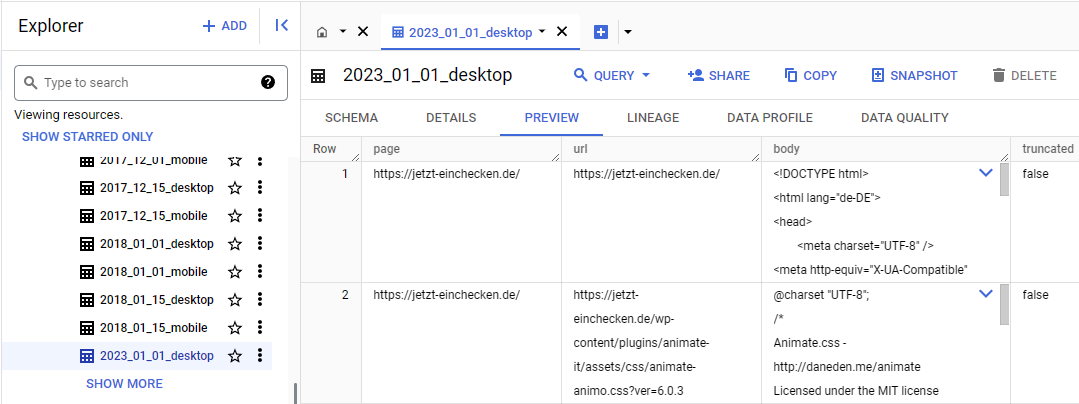
\includegraphics[scale=0.53]{obrazky-figures/bigquery_response_bodies.png}    
 \caption{\centering Pohľad na časť otvoreného okna s tabuľkou \code{2023\_01\_01\_desktop} v prostredí BigQuery Studio.}
 \label{img:bigquery-example-table}
\end{center}
\end{figure}

Prehľadávaním týchto dát a sledovaním obsahu HTTP hlavičiek je možné dopracovať sa k HTTP odpovediam s pravidlami technológie NEL.
Každú doménu, ktorá vo svojich odpovediach zaslala hlavičky \code{NEL} a \code{Report-To} je možné skúmať ako doménu s nasadeným monitorovaním NEL.

\subsection{Poplatky za používanie}

Čo sa platieb týka, BigQuery pre užívateľov poskytuje bezplatný plán s nastavenými limitmi pre využívanie konkrétnych funkcií.
\textbf{Bezplatný plán} zahŕňa 1TB procesnej kapacity dát a 10GB úložného priestoru pre vlastné dáta, pričom dochádza každý mesiac \mbox{k obnove týchto bezplatných zdrojov}.
Po prečerpaní kapacity uvedenej v tomto pláne je nutné akékoľvek ďalšie operácie doplatiť.
Zoznam spôsobov, akými je možné zaplatiť za navýšenie spomenutých kapacít je rozsiahly, no pre prípady použitia tejto práce je relevantný platobný plán zvaný On-demand.
\textbf{On-demand plán}, alebo platba podľa potreby sa vzťahuje na procesnú kapacitu, ktorá sa vyčerpáva vykonávaním operácií nad dátami.
Cena za 1TB kapacity je v čase písania práce \$6.25, pričom stále platí, že prvý terabajt je každý mesiac zadarmo \cite{google-bq-pricing}.
